\section{Linear Systems}
A linear system is a problem defined as follows: given $A \in \RR^{n \times n},\,b \in \RR^n$ we want to find, if possible, $x \in \RR^n$ such that $Ax = b$.

\subsection{Solvability}
If we consider $a^{(i)}$ the $i$-th column of matrix $A$, we can express the linear system as:
\begin{dmath*}
	Ax = a^{(1)}x_1 + a^{(2)}x_2 + \ldots + a^{(n)}x_n \stackrel{!}{=} b
\end{dmath*}

So a solution exists iff $b$ can be represented as a linear combination of columns of $A$, i.e. $b \in \op{span}(a^{(1)},\ldots,a^{(n)})$.
We already know that if $A$ has \emph{full-rank}\footnote{Its rank is the same as its dimension.}, then
\begin{equation*}
	\op{null}(A) \definedas \{ x \in \RR^n | Ax = 0 \} = \{0\}
\end{equation*}
so, by Grassmann's formula, $\op{dim}(Im(A)) = n$, therefore $b \in \op{span}(a^{(1)},\ldots,a^{(n)})$.

From now on, we will typically assume $A$ to be full rank.

\paragraph{How to compute a solution}
\todo{This is actually nonsensicle here, we should move it to where we actually talk about solving.}We may be tempted to proceed the naive way: $Ax = b \implies x = A^{-1}b$, but this turns out to be a very bad idea because:
\begin{itemize}
	\item Inverting a matrix in practice requires solving $n$ linear systems of the form $Ax = e_i$.
	\item Matrix inversion can be unstable.
\end{itemize}

\subsection{Conditioning of linear systems}
Let's see a simple $2 \times 2$ linear system, to get an idea on why resolution of linear system can be well or badly conditioned to different degrees. Consider:
\begin{align*}
	\begin{cases}
		a_{11} x_1 + a_{12} x_2 &= b_1\\
		a_{21} x_1 + a_{22} x_2 &= b_2
	\end{cases}
\end{align*}
In the ideal world, the solution of each equation is a mono-dimensional sub-space, i.e. a line. If we look at the intersection of these two lines, which is the combined solution of the linear system, we get a single point (a null-dimensional space).

However, if we take into account representation error on both $b$ and $A$, we get that the solution to each equation is not just a line, but more like a strip. That is, all the possible lines which are near enough the theoretical solution to be rounded (in some sense) to it are possible solutions.
\begin{figure}[H]
	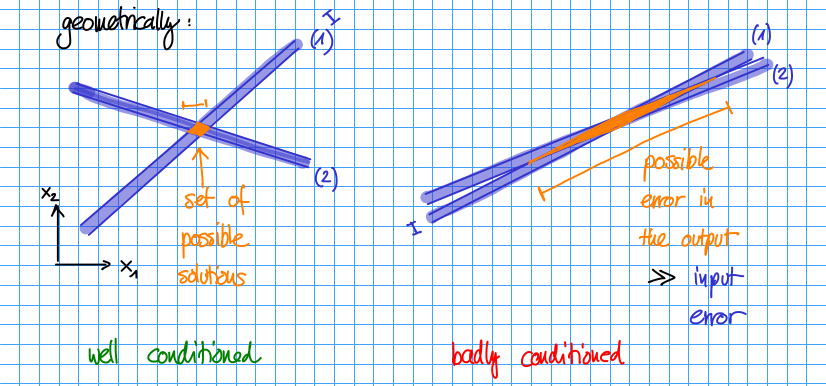
\includegraphics[width=\textwidth]{linSysConditioning}
\end{figure}
If we now consider the intersection of these two strips, we get an entire patch of the plane as possible solution set. We can see how the extent of this patch grows considerably the more the two solution strips tend to be parallel. This is, in simple terms, the conditioning of a linear system.
% EOF
